\documentclass[parskip=full]{scrartcl}


%%--PACKAGES-----------------------------------------------------
\usepackage[colorlinks=true,linkcolor=blue,urlcolor=black,bookmarksopen=true]{hyperref}
\usepackage[dvipsnames]{xcolor}
\usepackage[round]{natbib}
\usepackage{bookmark, amsfonts, amsthm, amsmath, amssymb, cancel, wrapfig, mathrsfs, enumitem}
\usepackage{tikz, circuitikz, subfig, subcaption, graphicx, float}
\bibliographystyle{plainnat}


%%--CORRECTIONS--------------------------------------------------
% \usepackage[switch, displaymath, mathlines]{lineno}
% \usepackage[allfiguresdraft]{draftfigure} % Disable pictures for fast rendering
% \linenumbers{}
% \counterwithin{equation}{subsection}
% \newcommand\inlinetag{\stepcounter{equation}\ (\theequation)}


%%--MATH---------------------------------------------------------
% Custom Letters
\def\N{\ensuremath{\mathbb{N}}}
\def\Z{\ensuremath{\mathbb{Z}}}
\def\Q{\ensuremath{\mathbb{Q}}}
\def\R{\ensuremath{\mathbb{R}}}
\def\S{\ensuremath{\mathbb{S}}}

\usepackage{bbm,dsfont}
\def\1{\ensuremath{\mathds{1}}}
\def\E{\ensuremath{\mathbf{E}}\:}
\def\P{\ensuremath{\mathbf{P}}}
\def\A{\ensuremath{\mathcal{A}}}
\def\AA{\ensuremath{\mathscr{A}}}
\def\CC{\ensuremath{\mathscr{C}}}

% Custom text commands
\def\Var{\ensuremath{\mathbf{Var}}\:}
\def\Bi{\ensuremath{\mathrm{Bi}}}
\def\Be{\ensuremath{\mathrm{Be}}}

% Theorems and more
\theoremstyle{definition}
\newtheorem{theorem}{Theorem}
\newtheorem{definition}{Definition}[theorem]
\newtheorem{corollary}{Corollary}[theorem]
\newtheorem{lemma}[theorem]{Lemma}
\newtheorem*{remark}{Remark}

% Custom Commands
\newcommand{\angles}[1]{\ensuremath{\left\langle}#1\ensuremath{\right\rangle} }
\newcommand{\floor}[1]{\ensuremath{\left\lfloor}#1\ensuremath{\right\rfloor} }
\newcommand{\ceil}[1]{\ensuremath{\left\lceil}#1\ensuremath{\right\rceil} }

% Section Numbering Fixes
\makeatletter
\renewcommand\thesection{}
\renewcommand\thesubsection{\@arabic\c@section.\@arabic\c@subsection}
\makeatother

% Title Info
\title{Stochastic Processes: Homework 1}
\author{Martín Prado}
\date{November 2023}
\publishers{Universidad de los Andes $-$ Bogotá Colombia}


%%--DOCUMENT-----------------------------------------------------
\begin{document}
\maketitle

% \tableofcontents

%%--WARNINGS-----------------------------------------------------
% chktex-file 9  - Half closed intervals
% chktex-file 17 - Half closed intervals
% chktex-file 36 - Space in front of parenthesis?

\section{Exercise 1}
Consider a sequence of i.i.d.~random variables ${(X_i)}_{i\in\N}$ with $\E X_i = 0$ and $\Var X_i = 1$ for every $i\in \N$.

\begin{enumerate}
    \item Show with th Law of Large Numbers that,
    \[ \lim_{n\to\infty} \|X_1,\ldots,X_n\|_2 - \sqrt{n} \to 0 \]
    \begin{enumerate}[label=(\alph*)]
        \item in $\mathbb{P}$,
        \item a.e.,
        \item in distribution,
        \item Show that if $X_i \in L^p$ for some $p>1$, then it converges in $L^q$ for every $q \in [1\leq p)$.
    \end{enumerate} 
    \item 
\end{enumerate}


\section{Exercise 2}
Prove the following theorem for $\tau = 0$ and $\tau = \infty$.

\begin{theorem}
    For any given $X$ with $F_X$ and $\overline{F}_X(x) = 1- F_X(x)$. Also let $M_n = X_{n:n}$. For $x\in \R$, if
    \begin{itemize}
        \item $\tau \in [0,\infty]$
        \item $(u_n)_{n\in\N}$ a non-decreasing sequence,
    \end{itemize}
    then the following items are equivalent,
    \begin{enumerate}
        \item $\lim_{n\to\infty} \P(M_n \leq u_n) = e^{-\tau}$
        \item $\lim_{n\to\infty} n \overline{F}_X(u_n) = \tau$.
    \end{enumerate}
\end{theorem}

\subsection*{Solution $\boldsymbol{\tau = 0}$}

\begin{itemize}
    \item $(2)\implies (1)$ If $n\cdot \ol{F}(u_n) \to 0$, then $\ol{F}(u_n) = o(1/n)$. Therefore,
    
    \[ \everymath{\displaystyle}
    \arraycolsep=1.8pt\def\arraystretch{1.8}
    \begin{array}{rll}
        \lim_n \P(M_n \leq u_n) & = \lim_n {F(u_n)}^n = \lim_n {(1-\ol{F}(u_n))}^n\\
        & = \lim_n {(1-o\left( \tfrac{1}{n} \right))}^n
    \end{array} \]
    What this means is that for every $\varepsilon > 0$, we will eventually have that 
    \[ \tfrac{-\varepsilon}{n} \leq  -\ol F(u_n) \leq \tfrac{\varepsilon}{n}. \]
    In particular, for every $\varepsilon > 0$,
    \[e^{-\varepsilon} \leq \lim_n {(1-\tfrac{\varepsilon}{n})}^n \leq \lim_n {(1-\ol{F}(u_n))}^n \leq \lim_n {(1+\tfrac{\varepsilon}{n})}^n = e^{\varepsilon}. \]
    Therefore, by making $\varepsilon$ go to $0$ we would obtain,
    \[ 1 \leq \lim_n {(1-\ol{F}(u_n))}^n \leq 1. \]
    \item $(1)\implies (2)$ Now, the hypothesis says that
    \[ \P(M_n \leq u_n) = \lim_n {(1-\ol{F}(u_n))}^n = 1. \]
    To prove that $\ol F(u_n) \to 0$, we use the same argument from the original proof. If $\liminf_n \ol{F}(u_n) = \alpha > 0$, then there exists a subsequence $u_{n_k} \subset u_n$ such that 
    \[ 1 = \lim_k {(1-\ol{F}(u_{n_k}))}^{n_k} \leq \lim_k {(1-\alpha)}^{n_k} = 0. \]
    With that in mind, we take logarithm at both sides to obtain
    \[ \lim_n n\cdot \ln((1-\ol{F}(u_{n}))) = 0.\]
    From Taylor's formula, $- \ln(1-x) = x + o(x)_{x\to 0+}$. Thus,
    \[ -0 = - \lim_n n\cdot \ln((1-\ol{F}(u_{n}))) = \lim_n n \ol{F}(u_{n}) \]
\end{itemize}

\subsection*{Solution $\boldsymbol{\tau = \infty}$}

\begin{itemize}
    \item $(2)\implies (1)$ $n\cdot \ol{F}(u_n) \to \infty$ is equivalent to
    \[ \lim_n \frac{1/\ol{F}(u_n)}{n} = 0. \]
    Which by definition means that $ \ol{F}(u_n)^{-1} = o(\tfrac{1}{n}) $. This implies that for every $\varepsilon>0$,
    \[ {\ol{F}(u_n)}^{-1} \leq \varepsilon n, \text{ (eventually)} \]
    \[ \implies -\ol{F}(u_n) \leq -\frac{\varepsilon'}{n} \]
    \[ \everymath{\displaystyle}
    \arraycolsep=1.8pt\def\arraystretch{1.8}
    \begin{array}{rll}
        \lim_n \P(M_n \leq u_n) & = \lim_n {F(u_n)}^n = \lim_n {(1-\ol{F}(u_n))}^n\\
        & \leq \lim_n {(1-\tfrac{\varepsilon}{n})}^n = e^{-\varepsilon}.
    \end{array} \]
    By making $\varepsilon \to \infty$, we can conclude that
    \[ \lim_n \P(M_n \leq u_n) = 0. \]
    \item $(1)\implies (2)$ Now, note that
    \[ \lim_n n\cdot \ln((1-\ol{F}(u_{n}))) = -\infty.\]
    Using Taylor's polynomial like we did in the case $\tau = 0$, will give us that
    \[ \lim_n n\cdot (\ol{F}(u_{n}) + o(\ol{F}(u_{n}))) = \infty.  \]
    Since, by definition, $\ol{F}(u_{n})$ dominates over $o(\ol{F}(u_{n}))$, we can conclude that
    \[  \lim_n n\cdot \ol{F}(u_{n}) = \infty.\]
\end{itemize}

\section{Exercise 3}
Let $f : [0,1]\to \R$ be a continuos function. Show with the Law of Large Numbers that there exists a sequence of polynomial ${(P_n)}_{n\in \N}$ such that $\deg(P_n) = n$ and,
\[ \lim_{n\to\infty} \sup_{x\in [0,1]} |f(x) - P_n(x)| = 0. \]

\subsection*{Solution}

Let $(X_n)_{n\in \N}$ be 

\newpage
\section{Exercise 4}
\begin{enumerate}
    \item Simulate 50 times, graph and compare the empirical distribution of $X_{i:6}$ for $i \in \{1,\ldots, 6\}$ with $X_k \sim U(0,1)$. Calculate the uniform distance $\|\cdot\|_\infty$ between the empirical and the real distributions.
    \item Simulate 50 times, graph and compare the empirical distribution of $X_{i:6}$ for $i \in \{1,\ldots, 6\}$ with $X_k \in F$, where
    \[ F = \begin{cases}
        0 & x\leq 1\\
        1- x^{-1} & x > 1.
    \end{cases} \]
    Calculate the uniform distance $\|\cdot\|_\infty$ between the empirical and the real distributions. Also calculate $f_{i:6}$, $F_{i:6}$ and determine which moments are finite.
\end{enumerate}


\subsection*{Solution Part 1}

We use the letter $F$ for the uniform distribution, $F_{i:n}$ for the order distribution of the $i-th$ element of the sample, and $F^*_{i:n}$ for the empirical distribution obtained from sampling $m$ times the $i-th$ order statistic. In fact, since we are working with the uniform distribution,
\[ F_{i:n}(x) = \text{Beta}_{(i,n-i+1)}(x). \]
The formula for the empirical distribution is the following:
\[ F^*_{i:n} = \frac{1}{m} \sum_{k = 1}^m \1\{X_{i:n}^{(k)} < x\}. \]
Finally, since $F_{i:n}(x)$ is monotonically increasing and $F^{*}_{i:n}(x)$ is piecewise constant, the formula for the uniform distance can be approximated by calculating $M$ times the following formula 
\[ \|F^*_{i:n} - F_{i:n}\|_\infty \approx \max_{k \in \{1,\ldots, M\}} |F_{i:n}(k/m) - F^*_{i:n}(k/m)|.\]
The exercise required $n = 6$ and $m = 50$, and I personally used $M = 5000$ for graphing and calculating the uniform distance.

\newpage

\begin{figure}[H]
    \centering
    \begin{tabular}{@{}c@{}}
        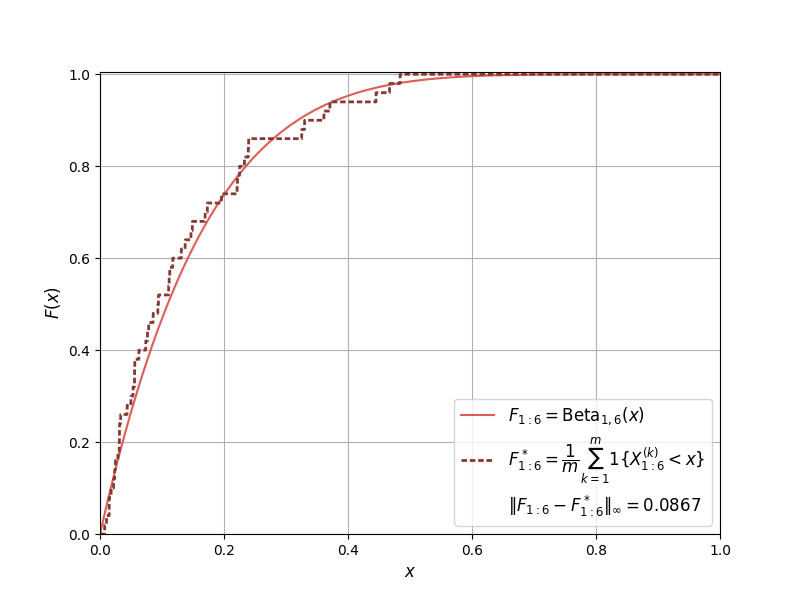
\includegraphics[trim={1.1cm 0.5cm 1.5cm 0cm}, clip,width=.46\linewidth]{../simulation/unif_order_1:6.png} \\
        $i = 1$
      \end{tabular}
    \begin{tabular}{@{}c@{}}
        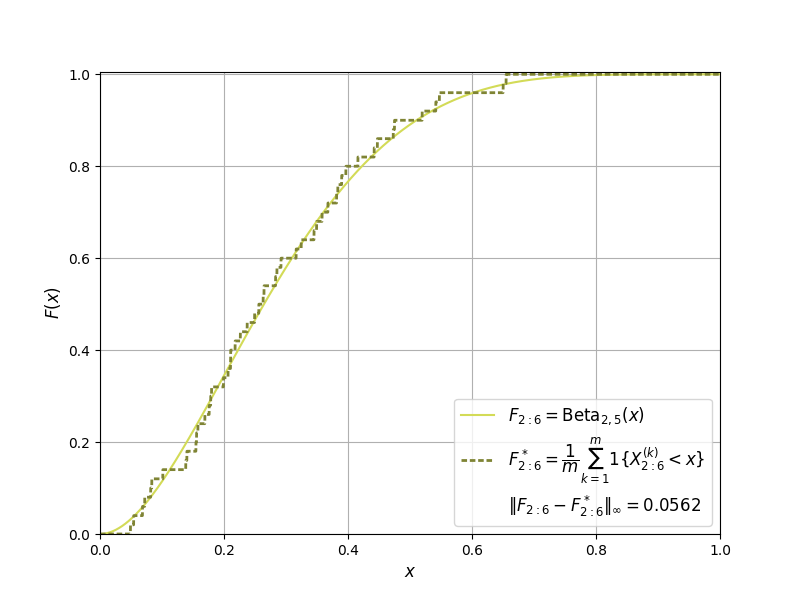
\includegraphics[trim={1.1cm 0.5cm 1.5cm 0cm}, clip,width=.46\linewidth]{../simulation/unif_order_2:6.png} \\
        $i = 2$
    \end{tabular}
    \begin{tabular}{@{}c@{}}
        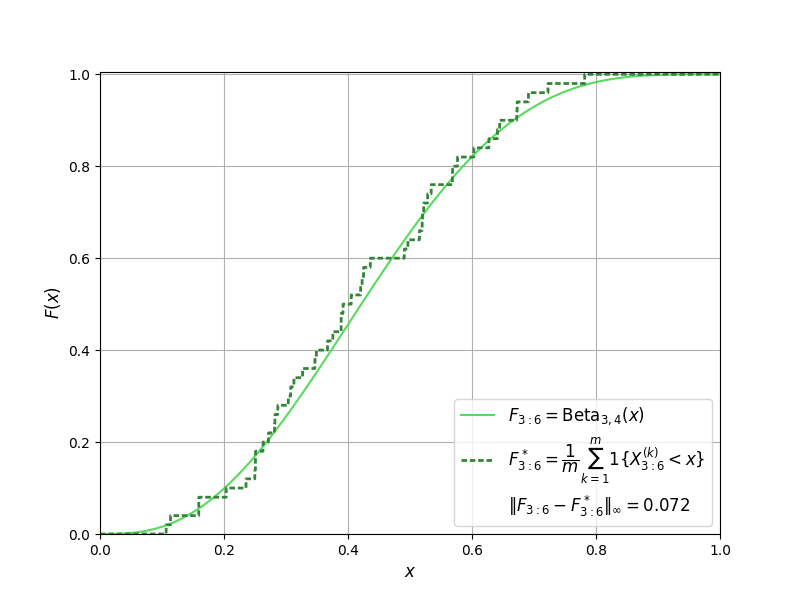
\includegraphics[trim={1.1cm 0.5cm 1.5cm 0cm}, clip,width=.46\linewidth]{../simulation/unif_order_3:6.png} \\
        $i = 3$
      \end{tabular}
    \begin{tabular}{@{}c@{}}
        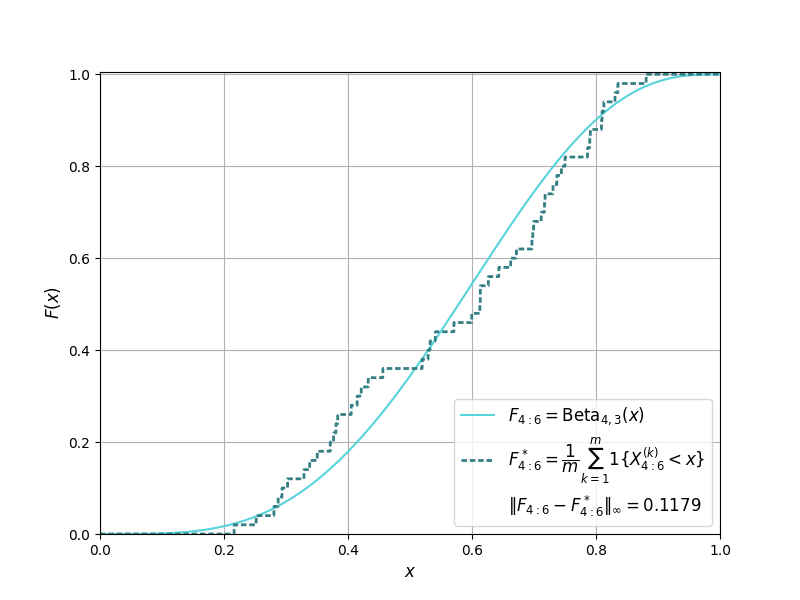
\includegraphics[trim={1.1cm 0.5cm 1.5cm 0cm}, clip,width=.46\linewidth]{../simulation/unif_order_4:6.png} \\
        $i = 4$
    \end{tabular}
    \begin{tabular}{@{}c@{}}
        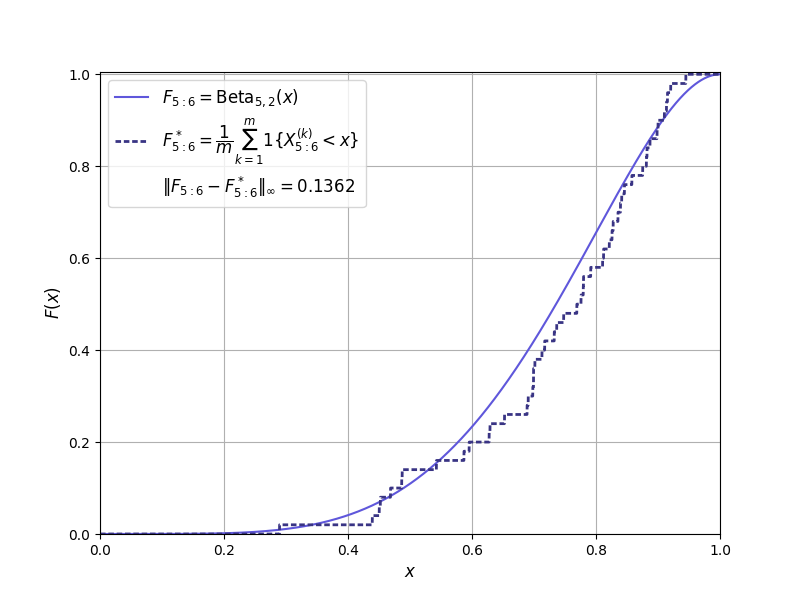
\includegraphics[trim={1.1cm 0.5cm 1.5cm 0cm}, clip,width=.46\linewidth]{../simulation/unif_order_5:6.png} \\
        $i = 5$
      \end{tabular}
    \begin{tabular}{@{}c@{}}
        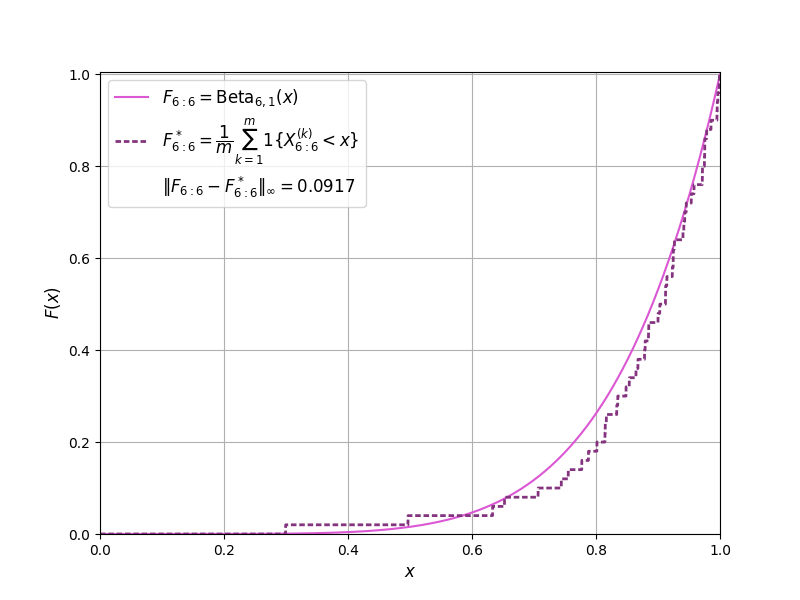
\includegraphics[trim={1.1cm 0.5cm 1.5cm 0cm}, clip,width=.46\linewidth]{../simulation/unif_order_6:6.png} \\
        $i = 6$
    \end{tabular}
    \caption{Simulation of the six order statistics for 6 samples of the Uniform Distribution}
\end{figure}

\newpage

\subsection*{Solution Part 2}

The distribution $F$ from part 2 is a type I Pareto distribution
\[ \text{Pareto}_{(\alpha, \sigma)}(x) = \begin{cases}
    0 & x\leq \sigma \\
    1- {\left( \frac{\sigma}{x} \right)}^{\alpha} & x > \sigma.
\end{cases} \]
with parameters $\alpha = \sigma = 1$. Therefore, the condition required for it to have the $k$-moment is that $k < \alpha$. Since $\alpha = 1$, it doesn't have any finite moments. Using the formula for the $i$-th statistic, we obtain
\[ F_{i:n} =  \]

\newpage

\begin{figure}[H]
    \centering
    \begin{tabular}{@{}c@{}}
        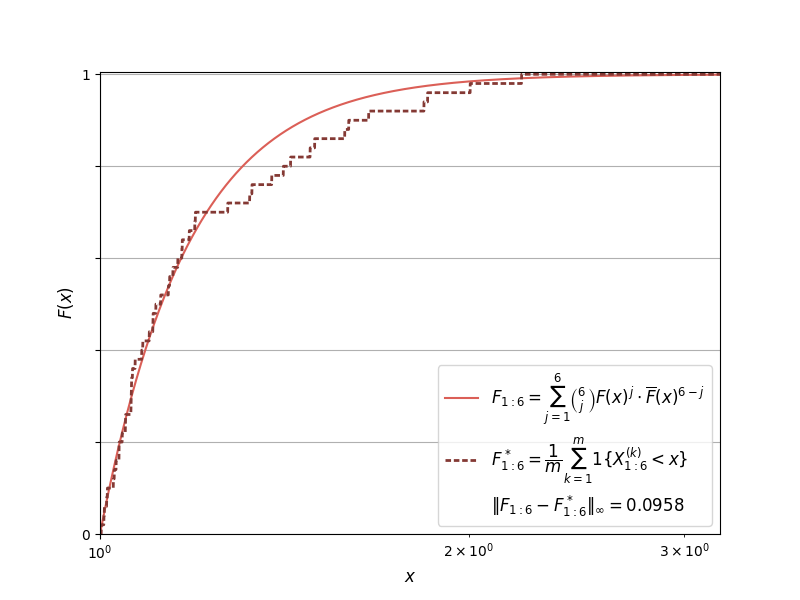
\includegraphics[trim={1.1cm 0.5cm 1.5cm 0cm}, clip,width=.46\linewidth]{../simulation/pareto_order_1:6.png} \\
        $i = 1$
      \end{tabular}
    \begin{tabular}{@{}c@{}}
        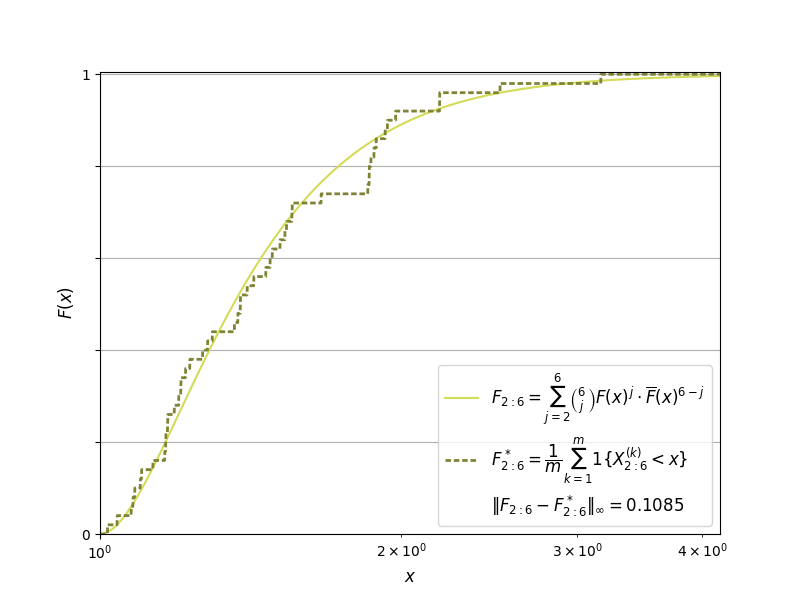
\includegraphics[trim={1.1cm 0.5cm 1.5cm 0cm}, clip,width=.46\linewidth]{../simulation/pareto_order_2:6.png} \\
        $i = 2$
    \end{tabular}
    \begin{tabular}{@{}c@{}}
        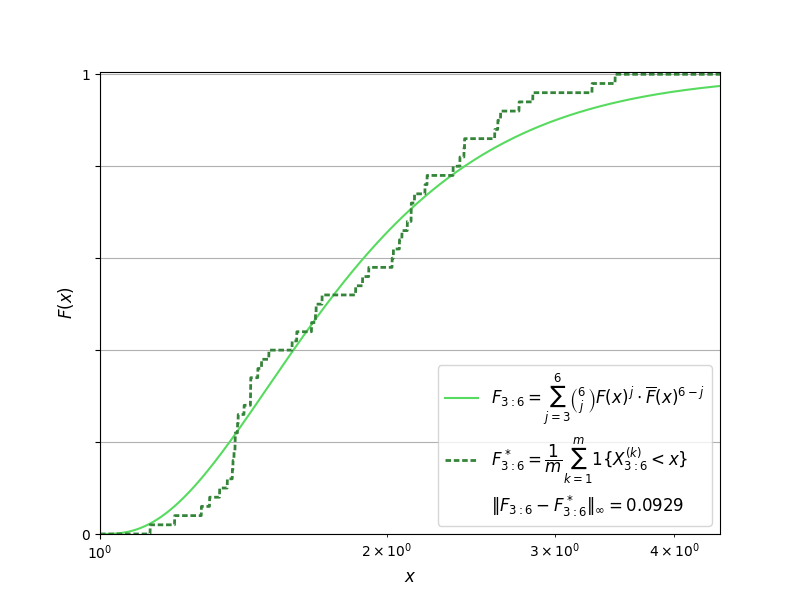
\includegraphics[trim={1.1cm 0.5cm 1.5cm 0cm}, clip,width=.46\linewidth]{../simulation/pareto_order_3:6.png} \\
        $i = 3$
      \end{tabular}
    \begin{tabular}{@{}c@{}}
        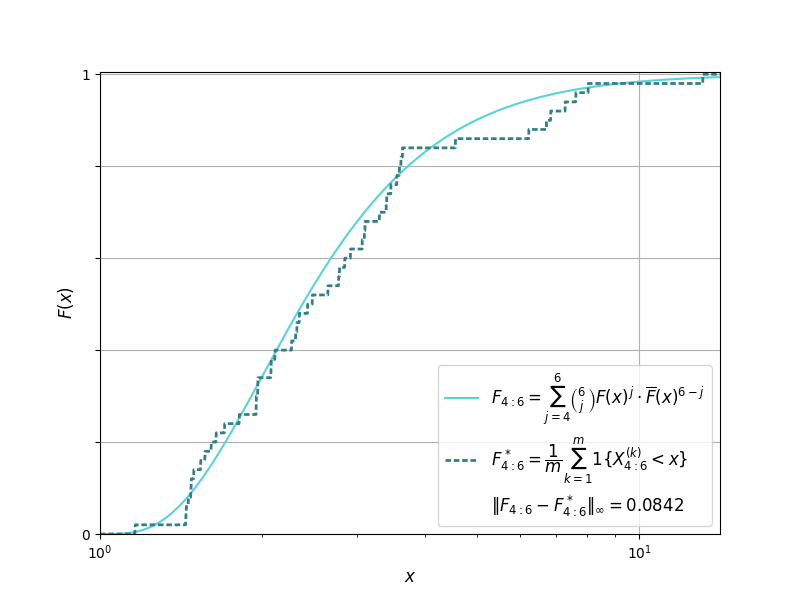
\includegraphics[trim={1.1cm 0.5cm 1.5cm 0cm}, clip,width=.46\linewidth]{../simulation/pareto_order_4:6.png} \\
        $i = 4$
    \end{tabular}
    \begin{tabular}{@{}c@{}}
        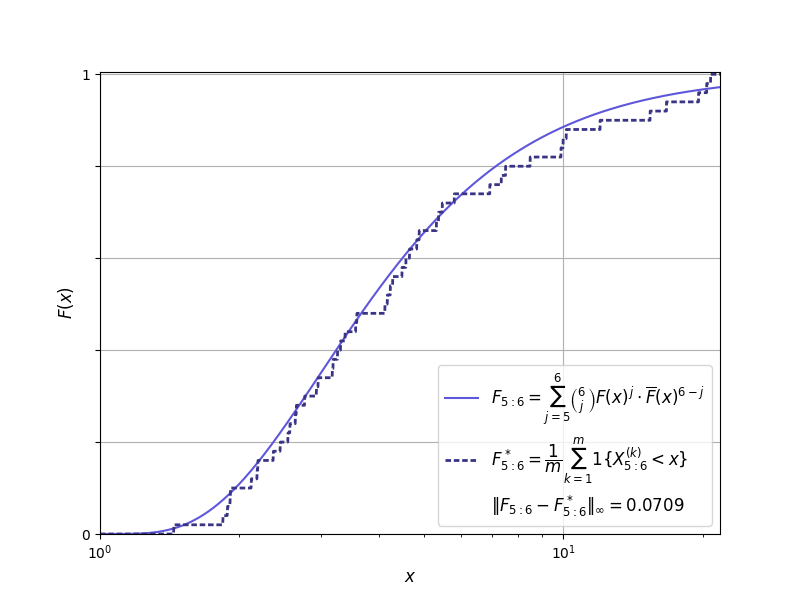
\includegraphics[trim={1.1cm 0.5cm 1.5cm 0cm}, clip,width=.46\linewidth]{../simulation/pareto_order_5:6.png} \\
        $i = 5$
      \end{tabular}
    \begin{tabular}{@{}c@{}}
        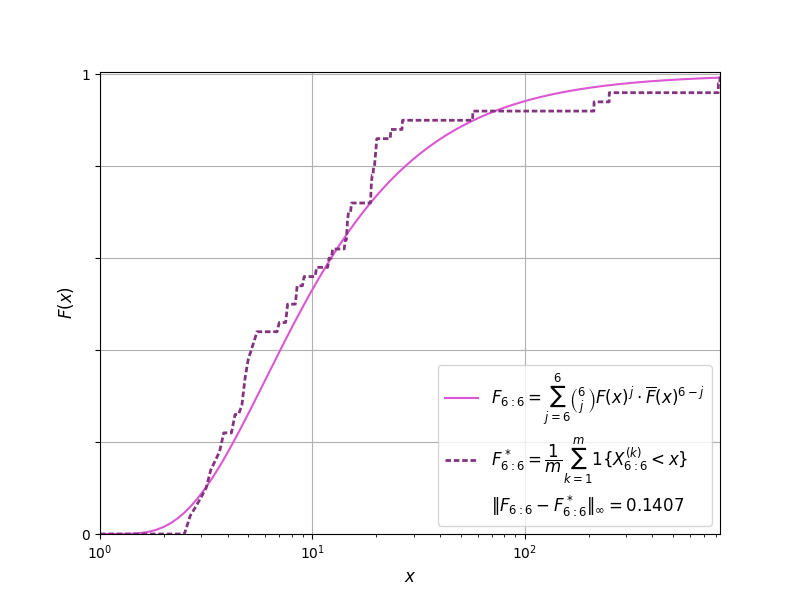
\includegraphics[trim={1.1cm 0.5cm 1.5cm 0cm}, clip,width=.46\linewidth]{../simulation/pareto_order_6:6.png} \\
        $i = 6$
    \end{tabular}
    \caption{Simulation of the six order statistics for 6 samples of the Pareto Distribution}
\end{figure}

% \bibliography{refs}

\end{document}